\section{Learning to adapt to opponents}
\label{sec:part3}

In the previous chapter we tried to create an algorithm to develop the default strategy for the APC. \\

The goal of this chapter is to further develop the strategy of APC to also adapt to the strategies of the opponents. This chapter will be mainly theoretical since it is based on the strategy of the previous chapter, which did not work.

\vspace{4mm}
\begin{statementBox2}{Problem statement 3}
How can one further develop a strategy for a poker computer to be able to adapt to the playing style of the opponent?
\end{statementBox2}
\vspace{4mm} 

In poker there is no such thing as a single optimal strategy. Every strategy has weaknesses and therefore the optimal strategy is one that takes advantage of the weaknesses of the strategies of the opponents. In order to take advantage of the opponents strategies one must first understand their strategy. In poker understanding the opponents is one of the most important key elements of the game. 

Once one understand the strategy of the opponent one has to adapt oneself's strategy.

\subsection{Design}
In order to learn the strategy of the opponents we try to model the player using player modeling, see section \ref{sec:pm}. 

In this section we will start by introducing the concept of player modeling. We then design the player model we wish to use for the APC and finally implement it as a subsystem called the poker player model.


\subsubsection{Player modeling}
\label{sec:pm}
Player modeling is a loosely defined concept and may vary from one context to another. The concept of player modeling is to make a computational model of a player. This model includes game related attributes, such as play style and preferences, as well as non-game related attributes, such as cultural background, gender, and personality. All decisions of the player are ultimately made on the basis of these attributes. 

Player modeling is used to describe or predict the players decisions, reasoning and reactions. In the field of artificial intelligences the human player is the most used model for developing computer players. Understanding the reason behind every choice of a player will not only bring a better understanding of the player but also a better understanding of the game and its mechanics.

Since the player model can easily become extremely extensive one normally only includes the relevant attributes of the player.

\subsubsection{Design of the player model}
It is crucial to figure out which attributes are relevant to the specific player model. When trying to model a player there is almost no limit to what could be included. Attributes such as state of mind, energy, and distractions affect the decision of every human player.  

We listed the attributes that we find most relevant for poker.

\begin{description}
\item[Aggressiveness] How often does the player tend to bet or raise.
\item[Tightness] How strictly does the player's actions reflect the strength of the hand. For instance, a tight player will play aggressive when having a strong hand and defensive or fold when having a weak hand. A loose player may bluff (play aggressive having a weak hand) and slow play (play defensive having a strong hand) a lot.
\item[Riskiness] How easy is it to push the player to fold. Risky players tend to fold less often and are therefore harder to bluff.
\item[Body language] Most human players unconsciously show emotions through their body language. The professional poker players can tell a lot about a players hole cards solely by looking at their body language.
\item[Time of decision making] The time a player use for each decision can show the confidence of the players choice. A fast decisions indicates an easy decision. 
\end{description}

Since our APC is targeted towards computer players as well as human players, it makes no sense to use attributes such as body language and the time of decision making to model the opponents. Those attributes only affect human players. Instead we will model the opponents using the attributes aggressiveness, tightness, and riskiness.

Aggressiveness is easy to find simply by looking at the actions of the opponent. 

Tightness is a bit more complicated as we need to know the hole cards of the player. We only track the tightness of rounds where the player make it to the showdown.

Riskiness is also complicated to measure as it is relative to the hole cards of the player. If a player has a weak hand and calls or raise, it is considered a risky play.  

The APC also need to be able to recognise if a player changes strategy during the game. To accomplish this we split each attribute into the two attributes: overall and recent. Overall covers every round throughout the game while recent only covers the last ten rounds.

The reason we choose ten games recent is because a player might get lucky and get several strong hole cards in a row. This may cause the player to play more aggressive than usual even though the player still uses the same strategy. This will result in a miss read by the player model. We found ten games to be high enough to avoid miss reads and also low enough to actually track changes in the players strategy.

Aggressiveness is also split into one additional attribute called current aggressiveness which is the player's previous aggressiveness of the current round.

We end using the following attributes attributes for our player model:
\begin{itemize}
\item Overall aggressiveness
\item Recent aggressiveness
\item Current aggressiveness
\item Overall tightness
\item Recent tightness
\item Overall riskiness
\item Recent riskiness
\end{itemize}

\subsubsection{Implementation of the player model?}
To model each player we have created a subsystem called the poker player model (PPM). The PPM is responsible for tracking the aggressiveness, tightness, and riskiness of a player.

A PPM object is created for each opponent and the PPM then tracks the attributes of the player when given the data from a round.\\

The aggressiveness of a round is found as:

\[Agg_{n} = \frac{AA_{n}}{TA_{n}}\]

$Agg_{n}$ is the aggressiveness of round $n$, $AA_{n}$ is the player's number of aggressive actions (bet or raise) of round $n$ and  $TA_{n}$ is the player's total number of actions in round $n$. This is found for every round. 

Overall-, recent-, and current aggressiveness is found as an average of all rounds, last ten rounds, and current round respectively.\\

The tightness of the player is found by backtracking the actions of the player after the round is finished. This is of cause only done for rounds that makes it to the showdown, since we otherwise do not know the hole cards of the player.

In order to determine if a player either bluff or slow play we first establish some boundaries based on the hand strength. 

We took a sample of 100 defensive action and 100 aggressive actions and plotted the data in figure \ref{fig:dist-act}. The boundary for bluffing (red line) shows that the players tends to play defensive below this line. Likewise the boundary for slow play (blue line) shows that the players tends to play aggressive above this line.

We define slow playing as playing defensive with a hand strength of more than 0,63.

We define bluffing as playing aggressive with a hand strength of less than 0,46.

We then find the tightness of a round $Ti_{n}$ using the formula:

\[Ti_{n} = \dfrac{Bluff_{n} + Slow_{n}}{TA_{n}}\]

Here $Bluff_{n}$ is the number of times the player bluffed, $Slow_{n}$ is the number of times the player slow played and $TA_{n}$ is the total number of actions.

We then find the 

\begin{figure}[H]
  \center
    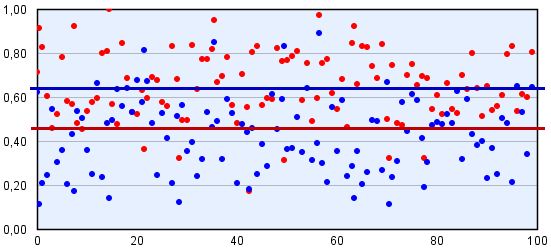
\includegraphics[scale=0.775]{images/modeling/action-dist.png}
  \caption{Distribution of actions in regards to the hand strength. Red dots indicates aggressive actions and blue dots defensive actions. The red line indicates the boundary for slow play and the blue line the boundary for bluffing. \label{fig:dist-act}}
\end{figure}





\subsection{Test}


\subsection{Discussion}

\subsection{Conclusion}
